% Options for packages loaded elsewhere
\PassOptionsToPackage{unicode}{hyperref}
\PassOptionsToPackage{hyphens}{url}
\PassOptionsToPackage{dvipsnames,svgnames,x11names}{xcolor}
%
\documentclass[
  letterpaper,
  DIV=11,
  numbers=noendperiod,
  oneside]{scrartcl}

\usepackage{amsmath,amssymb}
\usepackage{iftex}
\ifPDFTeX
  \usepackage[T1]{fontenc}
  \usepackage[utf8]{inputenc}
  \usepackage{textcomp} % provide euro and other symbols
\else % if luatex or xetex
  \usepackage{unicode-math}
  \defaultfontfeatures{Scale=MatchLowercase}
  \defaultfontfeatures[\rmfamily]{Ligatures=TeX,Scale=1}
\fi
\usepackage{lmodern}
\ifPDFTeX\else  
    % xetex/luatex font selection
\fi
% Use upquote if available, for straight quotes in verbatim environments
\IfFileExists{upquote.sty}{\usepackage{upquote}}{}
\IfFileExists{microtype.sty}{% use microtype if available
  \usepackage[]{microtype}
  \UseMicrotypeSet[protrusion]{basicmath} % disable protrusion for tt fonts
}{}
\makeatletter
\@ifundefined{KOMAClassName}{% if non-KOMA class
  \IfFileExists{parskip.sty}{%
    \usepackage{parskip}
  }{% else
    \setlength{\parindent}{0pt}
    \setlength{\parskip}{6pt plus 2pt minus 1pt}}
}{% if KOMA class
  \KOMAoptions{parskip=half}}
\makeatother
\usepackage{xcolor}
\usepackage[left=1in,marginparwidth=2.0666666666667in,textwidth=4.1333333333333in,marginparsep=0.3in]{geometry}
\setlength{\emergencystretch}{3em} % prevent overfull lines
\setcounter{secnumdepth}{5}
% Make \paragraph and \subparagraph free-standing
\ifx\paragraph\undefined\else
  \let\oldparagraph\paragraph
  \renewcommand{\paragraph}[1]{\oldparagraph{#1}\mbox{}}
\fi
\ifx\subparagraph\undefined\else
  \let\oldsubparagraph\subparagraph
  \renewcommand{\subparagraph}[1]{\oldsubparagraph{#1}\mbox{}}
\fi

\usepackage{color}
\usepackage{fancyvrb}
\newcommand{\VerbBar}{|}
\newcommand{\VERB}{\Verb[commandchars=\\\{\}]}
\DefineVerbatimEnvironment{Highlighting}{Verbatim}{commandchars=\\\{\}}
% Add ',fontsize=\small' for more characters per line
\usepackage{framed}
\definecolor{shadecolor}{RGB}{241,243,245}
\newenvironment{Shaded}{\begin{snugshade}}{\end{snugshade}}
\newcommand{\AlertTok}[1]{\textcolor[rgb]{0.68,0.00,0.00}{#1}}
\newcommand{\AnnotationTok}[1]{\textcolor[rgb]{0.37,0.37,0.37}{#1}}
\newcommand{\AttributeTok}[1]{\textcolor[rgb]{0.40,0.45,0.13}{#1}}
\newcommand{\BaseNTok}[1]{\textcolor[rgb]{0.68,0.00,0.00}{#1}}
\newcommand{\BuiltInTok}[1]{\textcolor[rgb]{0.00,0.23,0.31}{#1}}
\newcommand{\CharTok}[1]{\textcolor[rgb]{0.13,0.47,0.30}{#1}}
\newcommand{\CommentTok}[1]{\textcolor[rgb]{0.37,0.37,0.37}{#1}}
\newcommand{\CommentVarTok}[1]{\textcolor[rgb]{0.37,0.37,0.37}{\textit{#1}}}
\newcommand{\ConstantTok}[1]{\textcolor[rgb]{0.56,0.35,0.01}{#1}}
\newcommand{\ControlFlowTok}[1]{\textcolor[rgb]{0.00,0.23,0.31}{#1}}
\newcommand{\DataTypeTok}[1]{\textcolor[rgb]{0.68,0.00,0.00}{#1}}
\newcommand{\DecValTok}[1]{\textcolor[rgb]{0.68,0.00,0.00}{#1}}
\newcommand{\DocumentationTok}[1]{\textcolor[rgb]{0.37,0.37,0.37}{\textit{#1}}}
\newcommand{\ErrorTok}[1]{\textcolor[rgb]{0.68,0.00,0.00}{#1}}
\newcommand{\ExtensionTok}[1]{\textcolor[rgb]{0.00,0.23,0.31}{#1}}
\newcommand{\FloatTok}[1]{\textcolor[rgb]{0.68,0.00,0.00}{#1}}
\newcommand{\FunctionTok}[1]{\textcolor[rgb]{0.28,0.35,0.67}{#1}}
\newcommand{\ImportTok}[1]{\textcolor[rgb]{0.00,0.46,0.62}{#1}}
\newcommand{\InformationTok}[1]{\textcolor[rgb]{0.37,0.37,0.37}{#1}}
\newcommand{\KeywordTok}[1]{\textcolor[rgb]{0.00,0.23,0.31}{#1}}
\newcommand{\NormalTok}[1]{\textcolor[rgb]{0.00,0.23,0.31}{#1}}
\newcommand{\OperatorTok}[1]{\textcolor[rgb]{0.37,0.37,0.37}{#1}}
\newcommand{\OtherTok}[1]{\textcolor[rgb]{0.00,0.23,0.31}{#1}}
\newcommand{\PreprocessorTok}[1]{\textcolor[rgb]{0.68,0.00,0.00}{#1}}
\newcommand{\RegionMarkerTok}[1]{\textcolor[rgb]{0.00,0.23,0.31}{#1}}
\newcommand{\SpecialCharTok}[1]{\textcolor[rgb]{0.37,0.37,0.37}{#1}}
\newcommand{\SpecialStringTok}[1]{\textcolor[rgb]{0.13,0.47,0.30}{#1}}
\newcommand{\StringTok}[1]{\textcolor[rgb]{0.13,0.47,0.30}{#1}}
\newcommand{\VariableTok}[1]{\textcolor[rgb]{0.07,0.07,0.07}{#1}}
\newcommand{\VerbatimStringTok}[1]{\textcolor[rgb]{0.13,0.47,0.30}{#1}}
\newcommand{\WarningTok}[1]{\textcolor[rgb]{0.37,0.37,0.37}{\textit{#1}}}

\providecommand{\tightlist}{%
  \setlength{\itemsep}{0pt}\setlength{\parskip}{0pt}}\usepackage{longtable,booktabs,array}
\usepackage{calc} % for calculating minipage widths
% Correct order of tables after \paragraph or \subparagraph
\usepackage{etoolbox}
\makeatletter
\patchcmd\longtable{\par}{\if@noskipsec\mbox{}\fi\par}{}{}
\makeatother
% Allow footnotes in longtable head/foot
\IfFileExists{footnotehyper.sty}{\usepackage{footnotehyper}}{\usepackage{footnote}}
\makesavenoteenv{longtable}
\usepackage{graphicx}
\makeatletter
\def\maxwidth{\ifdim\Gin@nat@width>\linewidth\linewidth\else\Gin@nat@width\fi}
\def\maxheight{\ifdim\Gin@nat@height>\textheight\textheight\else\Gin@nat@height\fi}
\makeatother
% Scale images if necessary, so that they will not overflow the page
% margins by default, and it is still possible to overwrite the defaults
% using explicit options in \includegraphics[width, height, ...]{}
\setkeys{Gin}{width=\maxwidth,height=\maxheight,keepaspectratio}
% Set default figure placement to htbp
\makeatletter
\def\fps@figure{htbp}
\makeatother
\newlength{\cslhangindent}
\setlength{\cslhangindent}{1.5em}
\newlength{\csllabelwidth}
\setlength{\csllabelwidth}{3em}
\newlength{\cslentryspacingunit} % times entry-spacing
\setlength{\cslentryspacingunit}{\parskip}
\newenvironment{CSLReferences}[2] % #1 hanging-ident, #2 entry spacing
 {% don't indent paragraphs
  \setlength{\parindent}{0pt}
  % turn on hanging indent if param 1 is 1
  \ifodd #1
  \let\oldpar\par
  \def\par{\hangindent=\cslhangindent\oldpar}
  \fi
  % set entry spacing
  \setlength{\parskip}{#2\cslentryspacingunit}
 }%
 {}
\usepackage{calc}
\newcommand{\CSLBlock}[1]{#1\hfill\break}
\newcommand{\CSLLeftMargin}[1]{\parbox[t]{\csllabelwidth}{#1}}
\newcommand{\CSLRightInline}[1]{\parbox[t]{\linewidth - \csllabelwidth}{#1}\break}
\newcommand{\CSLIndent}[1]{\hspace{\cslhangindent}#1}

\KOMAoption{captions}{tableheading}
\makeatletter
\@ifpackageloaded{tcolorbox}{}{\usepackage[skins,breakable]{tcolorbox}}
\@ifpackageloaded{fontawesome5}{}{\usepackage{fontawesome5}}
\definecolor{quarto-callout-color}{HTML}{909090}
\definecolor{quarto-callout-note-color}{HTML}{0758E5}
\definecolor{quarto-callout-important-color}{HTML}{CC1914}
\definecolor{quarto-callout-warning-color}{HTML}{EB9113}
\definecolor{quarto-callout-tip-color}{HTML}{00A047}
\definecolor{quarto-callout-caution-color}{HTML}{FC5300}
\definecolor{quarto-callout-color-frame}{HTML}{acacac}
\definecolor{quarto-callout-note-color-frame}{HTML}{4582ec}
\definecolor{quarto-callout-important-color-frame}{HTML}{d9534f}
\definecolor{quarto-callout-warning-color-frame}{HTML}{f0ad4e}
\definecolor{quarto-callout-tip-color-frame}{HTML}{02b875}
\definecolor{quarto-callout-caution-color-frame}{HTML}{fd7e14}
\makeatother
\makeatletter
\makeatother
\makeatletter
\makeatother
\makeatletter
\@ifpackageloaded{caption}{}{\usepackage{caption}}
\AtBeginDocument{%
\ifdefined\contentsname
  \renewcommand*\contentsname{Table of contents}
\else
  \newcommand\contentsname{Table of contents}
\fi
\ifdefined\listfigurename
  \renewcommand*\listfigurename{List of Figures}
\else
  \newcommand\listfigurename{List of Figures}
\fi
\ifdefined\listtablename
  \renewcommand*\listtablename{List of Tables}
\else
  \newcommand\listtablename{List of Tables}
\fi
\ifdefined\figurename
  \renewcommand*\figurename{Figure}
\else
  \newcommand\figurename{Figure}
\fi
\ifdefined\tablename
  \renewcommand*\tablename{Table}
\else
  \newcommand\tablename{Table}
\fi
}
\@ifpackageloaded{float}{}{\usepackage{float}}
\floatstyle{ruled}
\@ifundefined{c@chapter}{\newfloat{codelisting}{h}{lop}}{\newfloat{codelisting}{h}{lop}[chapter]}
\floatname{codelisting}{Listing}
\newcommand*\listoflistings{\listof{codelisting}{List of Listings}}
\makeatother
\makeatletter
\@ifpackageloaded{caption}{}{\usepackage{caption}}
\@ifpackageloaded{subcaption}{}{\usepackage{subcaption}}
\makeatother
\makeatletter
\@ifpackageloaded{tcolorbox}{}{\usepackage[skins,breakable]{tcolorbox}}
\makeatother
\makeatletter
\@ifundefined{shadecolor}{\definecolor{shadecolor}{rgb}{.97, .97, .97}}
\makeatother
\makeatletter
\makeatother
\makeatletter
\@ifpackageloaded{sidenotes}{}{\usepackage{sidenotes}}
\@ifpackageloaded{marginnote}{}{\usepackage{marginnote}}
\makeatother
\makeatletter
\makeatother
\ifLuaTeX
  \usepackage{selnolig}  % disable illegal ligatures
\fi
\IfFileExists{bookmark.sty}{\usepackage{bookmark}}{\usepackage{hyperref}}
\IfFileExists{xurl.sty}{\usepackage{xurl}}{} % add URL line breaks if available
\urlstyle{same} % disable monospaced font for URLs
\hypersetup{
  pdftitle={Getting Started with Quarto},
  pdfauthor={Aidan Marnane},
  colorlinks=true,
  linkcolor={blue},
  filecolor={Maroon},
  citecolor={Blue},
  urlcolor={Blue},
  pdfcreator={LaTeX via pandoc}}

\title{Getting Started with Quarto}
\author{Aidan Marnane}
\date{2023-04-28}

\begin{document}
\maketitle
\ifdefined\Shaded\renewenvironment{Shaded}{\begin{tcolorbox}[boxrule=0pt, breakable, interior hidden, borderline west={3pt}{0pt}{shadecolor}, sharp corners, frame hidden, enhanced]}{\end{tcolorbox}}\fi

\renewcommand*\contentsname{Table of contents}
{
\hypersetup{linkcolor=}
\setcounter{tocdepth}{3}
\tableofcontents
}
In this document we will introduce a number of the key features Quarto
markdown files support. We will be following the
\href{https://quarto.org/docs/get-started/computations/vscode.html}{basic
tutorial} from Quarto as well as summarising some of the more advanced
features introduced in their comprehensive guide. \sidenote{\footnotesize Blog photo
  by
  \href{https://unsplash.com/@setyaki?utm_source=unsplash\&utm_medium=referral\&utm_content=creditCopyText}{Setyaki
  Irham} from
  \href{https://unsplash.com/photos/tfdff8Poebw?utm_source=unsplash\&utm_medium=referral\&utm_content=creditCopyText}{Unsplash}}

\hypertarget{what-is-quarto}{%
\subsection{What is Quarto?}\label{what-is-quarto}}

Quarto allows you to easily share and publish your
code/analysis/research through any of
markdown/\texttt{jupyter}/\texttt{knitr}. It is an extension of pandoc
and offers support for \texttt{python}/\texttt{R}/\texttt{Julia}.

\hypertarget{best-features}{%
\subsubsection{Best features}\label{best-features}}

\begin{itemize}
\tightlist
\item
  render \texttt{jupyter} notebooks
\item
  render markdown with code
\item
  advanced visual customisation - figures, layout, citations
\item
  create simple and easily customisable websites
\item
  Great integration with \href{https://code.visualstudio.com/}{VSCode}
  and \href{https://pages.github.com/}{Github Pages}.
\end{itemize}

\hypertarget{why-use-quarto}{%
\subsection{Why use quarto?}\label{why-use-quarto}}

Sharing jupyter notebooks is tedious. Either you share a link to a
prerendered notebook on github or you awkwardly convert to html/pdf with
a variety of tools.

\emph{The problem?} The conversion of a notebook is awkward. Often you
have to choose between removing all or including all the code. And while
the markdown support within \texttt{jupyt}er is good again the
customisation is limited.

Quarto solves this. It is a rendering tool that gives you a number of
options with customise how code, figures and text are arranged when
converting to \texttt{html} and \texttt{pdf}.

Even better it provides a new markdown format \texttt{.qmd} that allows
you to write \texttt{python} code within a markdown document (similar to
\texttt{R\ markdown}) or link to figures within a precomputed
\texttt{jupyter} notebook.

\hypertarget{writing-code}{%
\section{writing Code}\label{writing-code}}

\hypertarget{numpy}{%
\subsection{NumPy}\label{numpy}}

Create code blocks in markdown using
\texttt{\textasciigrave{}\textasciigrave{}\textasciigrave{}\{python\}}

\begin{Shaded}
\begin{Highlighting}[]

\NormalTok{::: \{.cell execution\_count=1\}}
\InformationTok{\textasciigrave{}\textasciigrave{}\textasciigrave{} \{.python .cell{-}code\}}
\ImportTok{import}\NormalTok{ numpy }\ImportTok{as}\NormalTok{ np}
\NormalTok{a }\OperatorTok{=}\NormalTok{ np.arange(}\DecValTok{15}\NormalTok{).reshape(}\DecValTok{3}\NormalTok{, }\DecValTok{5}\NormalTok{)}
\NormalTok{a}
\InformationTok{\textasciigrave{}\textasciigrave{}\textasciigrave{}}

\NormalTok{::: \{.cell{-}output .cell{-}output{-}display execution\_count=8\}}
\InformationTok{\textasciigrave{}\textasciigrave{}\textasciigrave{}}
\InformationTok{array([[ 0,  1,  2,  3,  4],}
\InformationTok{       [ 5,  6,  7,  8,  9],}
\InformationTok{       [10, 11, 12, 13, 14]])}
\InformationTok{\textasciigrave{}\textasciigrave{}\textasciigrave{}}
\NormalTok{:::}
\NormalTok{:::}

\end{Highlighting}
\end{Shaded}

\begin{Shaded}
\begin{Highlighting}[]
\ImportTok{import}\NormalTok{ numpy }\ImportTok{as}\NormalTok{ np}
\NormalTok{a }\OperatorTok{=}\NormalTok{ np.arange(}\DecValTok{15}\NormalTok{).reshape(}\DecValTok{3}\NormalTok{, }\DecValTok{5}\NormalTok{)}
\NormalTok{a}
\end{Highlighting}
\end{Shaded}

\begin{verbatim}
array([[ 0,  1,  2,  3,  4],
       [ 5,  6,  7,  8,  9],
       [10, 11, 12, 13, 14]])
\end{verbatim}

\hypertarget{matplotlib}{%
\subsection{Matplotlib}\label{matplotlib}}

Control how figures appear with comments
\texttt{\#\textbar{}\ keyword:\ value}. {[}\^{}:7{]}

\begin{Shaded}
\begin{Highlighting}[]

\NormalTok{::: \{.cell execution\_count=3\}}
\InformationTok{\textasciigrave{}\textasciigrave{}\textasciigrave{} \{.python .cell{-}code\}}
\ImportTok{import}\NormalTok{ matplotlib.pyplot }\ImportTok{as}\NormalTok{ plt}

\NormalTok{fig }\OperatorTok{=}\NormalTok{ plt.figure()}
\NormalTok{x }\OperatorTok{=}\NormalTok{ np.arange(}\DecValTok{10}\NormalTok{)}
\NormalTok{y }\OperatorTok{=} \FloatTok{2.5} \OperatorTok{*}\NormalTok{ np.sin(x }\OperatorTok{/} \DecValTok{20} \OperatorTok{*}\NormalTok{ np.pi)}
\NormalTok{yerr }\OperatorTok{=}\NormalTok{ np.linspace(}\FloatTok{0.05}\NormalTok{, }\FloatTok{0.2}\NormalTok{, }\DecValTok{10}\NormalTok{)}

\NormalTok{plt.errorbar(x, y }\OperatorTok{+} \DecValTok{3}\NormalTok{, yerr}\OperatorTok{=}\NormalTok{yerr, label}\OperatorTok{=}\StringTok{\textquotesingle{}both limits (default)\textquotesingle{}}\NormalTok{)}
\NormalTok{plt.errorbar(x, y }\OperatorTok{+} \DecValTok{2}\NormalTok{, yerr}\OperatorTok{=}\NormalTok{yerr, uplims}\OperatorTok{=}\VariableTok{True}\NormalTok{, label}\OperatorTok{=}\StringTok{\textquotesingle{}uplims=True\textquotesingle{}}\NormalTok{)}
\NormalTok{plt.errorbar(x, y }\OperatorTok{+} \DecValTok{1}\NormalTok{, yerr}\OperatorTok{=}\NormalTok{yerr, uplims}\OperatorTok{=}\VariableTok{True}\NormalTok{, lolims}\OperatorTok{=}\VariableTok{True}\NormalTok{,}
\NormalTok{             label}\OperatorTok{=}\StringTok{\textquotesingle{}uplims=True, lolims=True\textquotesingle{}}\NormalTok{)}

\NormalTok{upperlimits }\OperatorTok{=}\NormalTok{ [}\VariableTok{True}\NormalTok{, }\VariableTok{False}\NormalTok{] }\OperatorTok{*} \DecValTok{5}
\NormalTok{lowerlimits }\OperatorTok{=}\NormalTok{ [}\VariableTok{False}\NormalTok{, }\VariableTok{True}\NormalTok{] }\OperatorTok{*} \DecValTok{5}
\NormalTok{plt.errorbar(x, y, yerr}\OperatorTok{=}\NormalTok{yerr, uplims}\OperatorTok{=}\NormalTok{upperlimits, lolims}\OperatorTok{=}\NormalTok{lowerlimits,}
\NormalTok{             label}\OperatorTok{=}\StringTok{\textquotesingle{}subsets of uplims and lolims\textquotesingle{}}\NormalTok{)}

\NormalTok{plt.legend(loc}\OperatorTok{=}\StringTok{\textquotesingle{}lower right\textquotesingle{}}\NormalTok{)}
\NormalTok{plt.show(fig)}
\InformationTok{\textasciigrave{}\textasciigrave{}\textasciigrave{}}

\NormalTok{::: \{.cell{-}output .cell{-}output{-}display\}}
\AlertTok{![Errorbar limit selector](start{-}with{-}quarto\_files/figure{-}pdf/fig{-}limits{-}output{-}1.pdf)}\NormalTok{\{\#fig{-}limits fig{-}pos=\textquotesingle{}H\textquotesingle{}\}}
\NormalTok{:::}
\NormalTok{:::}

\end{Highlighting}
\end{Shaded}

\begin{Shaded}
\begin{Highlighting}[]
\ImportTok{import}\NormalTok{ matplotlib.pyplot }\ImportTok{as}\NormalTok{ plt}

\NormalTok{fig }\OperatorTok{=}\NormalTok{ plt.figure()}
\NormalTok{x }\OperatorTok{=}\NormalTok{ np.arange(}\DecValTok{10}\NormalTok{)}
\NormalTok{y }\OperatorTok{=} \FloatTok{2.5} \OperatorTok{*}\NormalTok{ np.sin(x }\OperatorTok{/} \DecValTok{20} \OperatorTok{*}\NormalTok{ np.pi)}
\NormalTok{yerr }\OperatorTok{=}\NormalTok{ np.linspace(}\FloatTok{0.05}\NormalTok{, }\FloatTok{0.2}\NormalTok{, }\DecValTok{10}\NormalTok{)}

\NormalTok{plt.errorbar(x, y }\OperatorTok{+} \DecValTok{3}\NormalTok{, yerr}\OperatorTok{=}\NormalTok{yerr, label}\OperatorTok{=}\StringTok{\textquotesingle{}both limits (default)\textquotesingle{}}\NormalTok{)}
\NormalTok{plt.errorbar(x, y }\OperatorTok{+} \DecValTok{2}\NormalTok{, yerr}\OperatorTok{=}\NormalTok{yerr, uplims}\OperatorTok{=}\VariableTok{True}\NormalTok{, label}\OperatorTok{=}\StringTok{\textquotesingle{}uplims=True\textquotesingle{}}\NormalTok{)}
\NormalTok{plt.errorbar(x, y }\OperatorTok{+} \DecValTok{1}\NormalTok{, yerr}\OperatorTok{=}\NormalTok{yerr, uplims}\OperatorTok{=}\VariableTok{True}\NormalTok{, lolims}\OperatorTok{=}\VariableTok{True}\NormalTok{,}
\NormalTok{             label}\OperatorTok{=}\StringTok{\textquotesingle{}uplims=True, lolims=True\textquotesingle{}}\NormalTok{)}

\NormalTok{upperlimits }\OperatorTok{=}\NormalTok{ [}\VariableTok{True}\NormalTok{, }\VariableTok{False}\NormalTok{] }\OperatorTok{*} \DecValTok{5}
\NormalTok{lowerlimits }\OperatorTok{=}\NormalTok{ [}\VariableTok{False}\NormalTok{, }\VariableTok{True}\NormalTok{] }\OperatorTok{*} \DecValTok{5}
\NormalTok{plt.errorbar(x, y, yerr}\OperatorTok{=}\NormalTok{yerr, uplims}\OperatorTok{=}\NormalTok{upperlimits, lolims}\OperatorTok{=}\NormalTok{lowerlimits,}
\NormalTok{             label}\OperatorTok{=}\StringTok{\textquotesingle{}subsets of uplims and lolims\textquotesingle{}}\NormalTok{)}

\NormalTok{plt.legend(loc}\OperatorTok{=}\StringTok{\textquotesingle{}lower right\textquotesingle{}}\NormalTok{)}
\NormalTok{plt.show(fig)}
\end{Highlighting}
\end{Shaded}

\begin{figure}[H]

{\centering 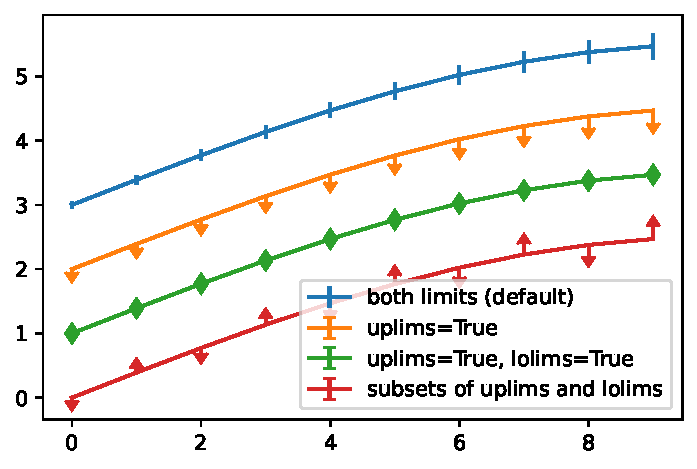
\includegraphics{start-with-quarto_files/figure-pdf/fig-limits-eg-output-1.pdf}

}

\caption{\label{fig-limits-eg}Errorbar limit selector}

\end{figure}

\hypertarget{plotly}{%
\subsection{Plotly}\label{plotly}}

\hypertarget{without-options}{%
\subsubsection{without options}\label{without-options}}

\begin{Shaded}
\begin{Highlighting}[]
\ImportTok{import}\NormalTok{ plotly.express }\ImportTok{as}\NormalTok{ px}
\ImportTok{import}\NormalTok{ plotly.io }\ImportTok{as}\NormalTok{ pio}
\NormalTok{gapminder }\OperatorTok{=}\NormalTok{ px.data.gapminder()}
\NormalTok{gapminder2007 }\OperatorTok{=}\NormalTok{ gapminder.query(}\StringTok{"year == 2007"}\NormalTok{)}
\NormalTok{fig }\OperatorTok{=}\NormalTok{ px.scatter(gapminder2007, }
\NormalTok{                 x}\OperatorTok{=}\StringTok{"gdpPercap"}\NormalTok{, y}\OperatorTok{=}\StringTok{"lifeExp"}\NormalTok{, color}\OperatorTok{=}\StringTok{"continent"}\NormalTok{, }
\NormalTok{                 size}\OperatorTok{=}\StringTok{"pop"}\NormalTok{, size\_max}\OperatorTok{=}\DecValTok{60}\NormalTok{,}
\NormalTok{                 hover\_name}\OperatorTok{=}\StringTok{"country"}\NormalTok{)}
\NormalTok{fig.show()}
\end{Highlighting}
\end{Shaded}

\begin{verbatim}
Unable to display output for mime type(s): text/html
\end{verbatim}

\begin{verbatim}
Unable to display output for mime type(s): text/html
\end{verbatim}

\hypertarget{with-options}{%
\subsubsection{With Options}\label{with-options}}

\begin{Shaded}
\begin{Highlighting}[]
\ImportTok{import}\NormalTok{ plotly.express }\ImportTok{as}\NormalTok{ px}
\ImportTok{import}\NormalTok{ plotly.io }\ImportTok{as}\NormalTok{ pio}
\NormalTok{gapminder }\OperatorTok{=}\NormalTok{ px.data.gapminder()}
\NormalTok{gapminder2007 }\OperatorTok{=}\NormalTok{ gapminder.query(}\StringTok{"year == 2007"}\NormalTok{)}
\NormalTok{fig }\OperatorTok{=}\NormalTok{ px.scatter(gapminder2007, }
\NormalTok{                 x}\OperatorTok{=}\StringTok{"gdpPercap"}\NormalTok{, y}\OperatorTok{=}\StringTok{"lifeExp"}\NormalTok{, color}\OperatorTok{=}\StringTok{"continent"}\NormalTok{, }
\NormalTok{                 size}\OperatorTok{=}\StringTok{"pop"}\NormalTok{, size\_max}\OperatorTok{=}\DecValTok{60}\NormalTok{,}
\NormalTok{                 hover\_name}\OperatorTok{=}\StringTok{"country"}\NormalTok{)}
\NormalTok{fig.show()}

\NormalTok{gapminder1957 }\OperatorTok{=}\NormalTok{ gapminder.query(}\StringTok{"year == 1957"}\NormalTok{)}
\NormalTok{fig }\OperatorTok{=}\NormalTok{ px.scatter(gapminder1957, }
\NormalTok{                 x}\OperatorTok{=}\StringTok{"gdpPercap"}\NormalTok{, y}\OperatorTok{=}\StringTok{"lifeExp"}\NormalTok{, color}\OperatorTok{=}\StringTok{"continent"}\NormalTok{, }
\NormalTok{                 size}\OperatorTok{=}\StringTok{"pop"}\NormalTok{, size\_max}\OperatorTok{=}\DecValTok{60}\NormalTok{,}
\NormalTok{                 hover\_name}\OperatorTok{=}\StringTok{"country"}\NormalTok{)}
\NormalTok{fig.show()}
\end{Highlighting}
\end{Shaded}

\begin{figure*}

\begin{minipage}[t]{0.50\linewidth}

{\centering 

\begin{verbatim}
Unable to display output for mime type(s): text/html
\end{verbatim}

}

\subcaption{\label{fig-gapminder-1}Gapminder: 1957}
\end{minipage}%
%
\begin{minipage}[t]{0.50\linewidth}

{\centering 

\begin{verbatim}
Unable to display output for mime type(s): text/html
\end{verbatim}

}

\subcaption{\label{fig-gapminder-2}Gapminder: 2007}
\end{minipage}%

\caption{\label{fig-gapminder}Life Expectancy and GDP}

\end{figure*}

\hypertarget{from-notebooks}{%
\subsection{From Notebooks}\label{from-notebooks}}

It is simple to embed plots from precomputed notebooks and include a
link.

\begin{verbatim}

\end{verbatim}

\begin{figure}

{\centering 

\begin{verbatim}
alt.Chart(...)
\end{verbatim}

}

\caption{\label{fig-bill-scatter}A scatterplot of bill dimensions for
penguins, made with Altair.}

\end{figure}

\begin{verbatim}

\end{verbatim}

\begin{figure}

\begin{minipage}[t]{0.50\linewidth}

{\centering 

\raisebox{-\height}{

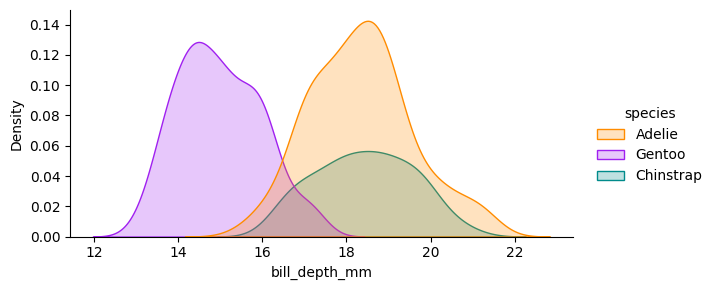
\includegraphics{start-with-quarto_files/figure-latex/fig-bill-marginal-output-1.png}

}

}

\subcaption{\label{fig-bill-marginal-1}Gentoo penguins tend to have
thinner bills,}
\end{minipage}%
%
\begin{minipage}[t]{0.50\linewidth}

{\centering 

\raisebox{-\height}{

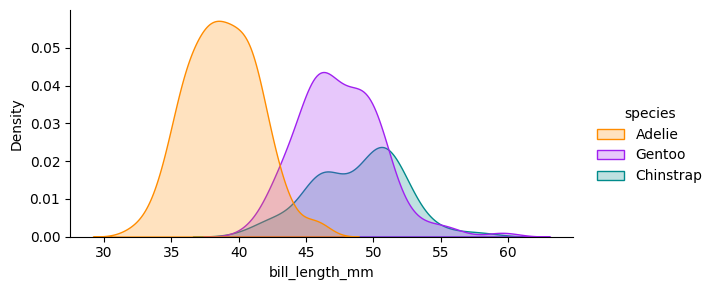
\includegraphics{start-with-quarto_files/figure-latex/fig-bill-marginal-output-2.png}

}

}

\subcaption{\label{fig-bill-marginal-2}and Adelie penguins tend to have
shorter bills.}
\end{minipage}%

\caption{\label{fig-bill-marginal}Marginal distributions of bill
dimensions}

\end{figure}

You can also include the code by specifying \texttt{echo=true} in the
call.

\begin{verbatim}

\end{verbatim}

\begin{Shaded}
\begin{Highlighting}[]
\NormalTok{penguins.groupby(}\StringTok{"species"}\NormalTok{).size().reset\_index(name }\OperatorTok{=} \StringTok{"count"}\NormalTok{)}
\end{Highlighting}
\end{Shaded}

\hypertarget{species-counts}{}
\begin{longtable}[]{@{}lll@{}}
\toprule\noalign{}
& species & count \\
\midrule\noalign{}
\endhead
\bottomrule\noalign{}
\endlastfoot
0 & Adelie & 152 \\
1 & Chinstrap & 68 \\
2 & Gentoo & 124 \\
\end{longtable}

You can control how the link to the notebook appears in the title
metadata \sidenote{\footnotesize See the
  \href{https://quarto.org/docs/authoring/notebook-embed.html}{notebook
  embedding tutorial} for more info}

\begin{verbatim}
notebook-view:
  - notebook: penguins.ipynb
    title: "Plots and Computations"
\end{verbatim}

\hypertarget{rendering-code}{%
\subsection{rendering code}\label{rendering-code}}

There are a number of ways to control the rendering of code. For
example, if you have a notebook with some code that takes a long time to
run you won't want to recompute it everytime you change formatting.
There are many options to control this behaviour. \sidenote{\footnotesize see the
  \href{https://quarto.org/docs/computations/python.html}{python
  tutorial} for a more in depth explanation}

\begin{verbatim}
execute:
  freeze: true 
\end{verbatim}

\hypertarget{formatting}{%
\section{Formatting}\label{formatting}}

\hypertarget{callout-blocks}{%
\subsection{callout blocks}\label{callout-blocks}}

Quarto has nice control for adding note blocks. There are five formats
\sidenote{\footnotesize See
  \href{https://quarto.org/docs/authoring/callouts.html}{their tutorial}
  for a more in depth explanation} - note - warning - important - tip -
caution

\begin{verbatim}
::: {.callout-note}
Note that there are five types of callouts, including:
`note`, `warning`, `important`, `tip`, and `caution`.
:::

::: {.callout-tip}
## Tip with Title

This is an example of a callout with a title. See [their tutorial](https://quarto.org/docs/authoring/callouts.html) for a more in depth explanation
:::

::: {.callout-caution collapse="true"}
## Expand To Learn About Collapse

This is an example of a 'folded' caution callout that can be expanded by the user. You can use `collapse="true"` to collapse it by default or `collapse="false"` to make a collapsible callout that is expanded by default.
:::
\end{verbatim}

\begin{tcolorbox}[enhanced jigsaw, opacitybacktitle=0.6, toprule=.15mm, arc=.35mm, opacityback=0, bottomrule=.15mm, coltitle=black, colbacktitle=quarto-callout-note-color!10!white, breakable, title=\textcolor{quarto-callout-note-color}{\faInfo}\hspace{0.5em}{Note}, colframe=quarto-callout-note-color-frame, left=2mm, colback=white, leftrule=.75mm, bottomtitle=1mm, toptitle=1mm, titlerule=0mm, rightrule=.15mm]

Note that there are five types of callouts, including: \texttt{note},
\texttt{warning}, \texttt{important}, \texttt{tip}, and
\texttt{caution}.

\end{tcolorbox}

\begin{tcolorbox}[enhanced jigsaw, opacitybacktitle=0.6, toprule=.15mm, arc=.35mm, opacityback=0, bottomrule=.15mm, coltitle=black, colbacktitle=quarto-callout-tip-color!10!white, breakable, title=\textcolor{quarto-callout-tip-color}{\faLightbulb}\hspace{0.5em}{Tip with Title}, colframe=quarto-callout-tip-color-frame, left=2mm, colback=white, leftrule=.75mm, bottomtitle=1mm, toptitle=1mm, titlerule=0mm, rightrule=.15mm]

This is an example of a callout with a title.

\end{tcolorbox}

\begin{tcolorbox}[enhanced jigsaw, opacitybacktitle=0.6, toprule=.15mm, arc=.35mm, opacityback=0, bottomrule=.15mm, coltitle=black, colbacktitle=quarto-callout-caution-color!10!white, breakable, title=\textcolor{quarto-callout-caution-color}{\faFire}\hspace{0.5em}{Expand To Learn About Collapse}, colframe=quarto-callout-caution-color-frame, left=2mm, colback=white, leftrule=.75mm, bottomtitle=1mm, toptitle=1mm, titlerule=0mm, rightrule=.15mm]

This is an example of a `folded' caution callout that can be expanded by
the user. You can use \texttt{collapse="true"} to collapse it by default
or \texttt{collapse="false"} to make a collapsible callout that is
expanded by default.

\end{tcolorbox}

\hypertarget{cross-referencing}{%
\subsection{Cross referencing}\label{cross-referencing}}

\begin{Shaded}
\begin{Highlighting}[]
\ImportTok{import}\NormalTok{ matplotlib.pyplot }\ImportTok{as}\NormalTok{ plt}
\NormalTok{plt.plot([}\DecValTok{1}\NormalTok{,}\DecValTok{23}\NormalTok{,}\DecValTok{2}\NormalTok{,}\DecValTok{4}\NormalTok{])}
\NormalTok{plt.show()}
\end{Highlighting}
\end{Shaded}

\begin{figure}[H]

{\centering 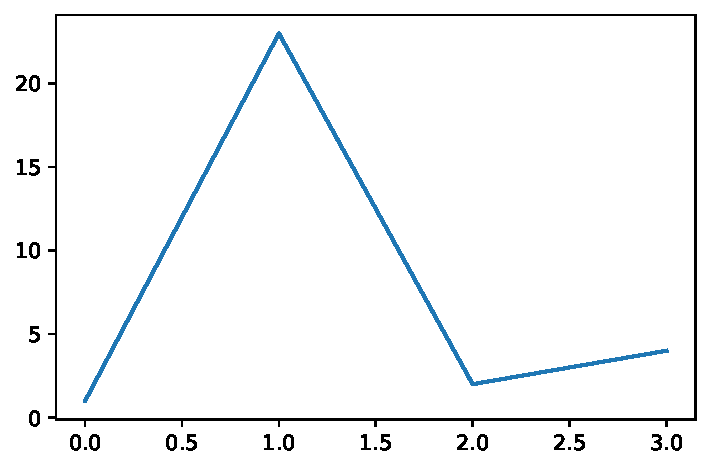
\includegraphics{start-with-quarto_files/figure-pdf/fig-line-plot-output-1.pdf}

}

\caption{\label{fig-line-plot}A line plot}

\end{figure}

This is a cross reference to our figure Figure~\ref{fig-line-plot} with
\texttt{@fig-line-plot}. We can also reference the matplotlib figure
above Figure~\ref{fig-limits-eg} \texttt{@fig-limits-eg}.

\begin{tcolorbox}[enhanced jigsaw, opacitybacktitle=0.6, toprule=.15mm, arc=.35mm, opacityback=0, bottomrule=.15mm, coltitle=black, colbacktitle=quarto-callout-note-color!10!white, breakable, title=\textcolor{quarto-callout-note-color}{\faInfo}\hspace{0.5em}{Note}, colframe=quarto-callout-note-color-frame, left=2mm, colback=white, leftrule=.75mm, bottomtitle=1mm, toptitle=1mm, titlerule=0mm, rightrule=.15mm]

You must start your label with \texttt{fig-} e.g.~\texttt{fig-line-plot}
for the cross reference to work.

\end{tcolorbox}

\hypertarget{citations}{%
\subsection{Citations}\label{citations}}

You can include citations by including a bibliography.

For example, Antoine et al produced some sick work (Lain et al. 2022).

Add a path to your bibliography in the title metadata

\begin{verbatim}

---
title: "My Document"
bibliography: references.bib
---
\end{verbatim}

You can customise citation style and more.\sidenote{\footnotesize Footnotes are also
  possible. For more guidance see the
  \href{https://quarto.org/docs/authoring/footnotes-and-citations.html}{quarto
  tutorial}}

\begin{verbatim}

---
title: "My Document"
bibliography: references.bib
csl: nature.csl
---
\end{verbatim}

\begin{tcolorbox}[enhanced jigsaw, opacitybacktitle=0.6, toprule=.15mm, arc=.35mm, opacityback=0, bottomrule=.15mm, coltitle=black, colbacktitle=quarto-callout-note-color!10!white, breakable, title=\textcolor{quarto-callout-note-color}{\faInfo}\hspace{0.5em}{Note}, colframe=quarto-callout-note-color-frame, left=2mm, colback=white, leftrule=.75mm, bottomtitle=1mm, toptitle=1mm, titlerule=0mm, rightrule=.15mm]

You can download csl files from the
\href{https://github.com/citation-style-language/styles}{CSL repo}.
nature.csl was taken from
\href{https://github.com/citation-style-language/styles/blob/master/nature.csl}{here}
(there are so many I had to search to get it.)

\end{tcolorbox}

Citation can also be placed in the margin by adding

\begin{verbatim}
citation-location: margin
\end{verbatim}

\hypertarget{equations}{%
\subsection{Equations}\label{equations}}

We can also write equations.

They can be placed inline
\(\frac{d}{dx}\left( \int_{a}^{x} f(u)\,du\right)=f(x).\)
\texttt{\$\textbackslash{}frac\{d\}\{dx\}\textbackslash{}left(\ \textbackslash{}int\_\{a\}\^{}\{x\}\ f(u)\textbackslash{},du\textbackslash{}right)=f(x).\$}.

They can be placed centrally.

\begin{verbatim}
$$\frac{d}{dx}\left( \int_{a}^{x} f(u)\,du\right)=f(x).$$
\end{verbatim}

\[\frac{d}{dx}\left( \int_{a}^{x} f(u)\,du\right)=f(x).\]

But they can also be placed in the margin

\begin{verbatim}
::: {.column-margin}
We know from *the first fundamental theorem of calculus* that for $x$ in $[a, b]$:


$$\frac{d}{dx}\left( \int_{a}^{x} f(u)\,du\right)=f(x).$$

:::
\end{verbatim}

\marginnote{\begin{footnotesize}

We know from \emph{the first fundamental theorem of calculus} that for
\(x\) in \([a, b]\):

\[\frac{d}{dx}\left( \int_{a}^{x} f(u)\,du\right)=f(x).\]

\end{footnotesize}}

\hypertarget{refs}{}
\begin{CSLReferences}{1}{0}
\leavevmode\vadjust pre{\hypertarget{ref-alain-2022}{}}%
Lain, Antoine, Wonjin Yoon, Hyunjae Kim, Jaewoo Kang, and Ian Simpson.
2022. {``{KU}{\_}{ED} at {S}ocial{D}is{NER}: Extracting Disease Mentions
in Tweets Written in {S}panish.''} In \emph{Proceedings of the Seventh
Workshop on Social Media Mining for Health Applications, Workshop {\&}
Shared Task}, 78--80. Gyeongju, Republic of Korea: Association for
Computational Linguistics.
\url{https://aclanthology.org/2022.smm4h-1.23}.

\end{CSLReferences}



\end{document}
